\thispagestyle{empty}
\null
\vfill
\begin{center}
   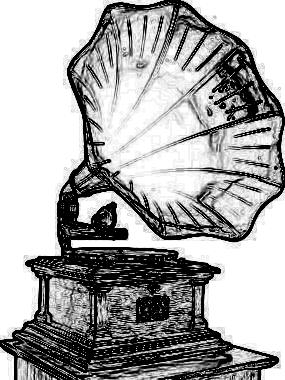
\includegraphics[width=0.8\textwidth, frame]{res/klassiskavisor.jpg}
   \section{Klassiska visor}
\end{center}
\vfill
\newpage



\newpage
\subsection{Du gamla du fria}
\textit{Mel: Du gamla du fria}\\
\index[alfa]{Du gamla du fria}
\index[anfa]{Du gamla, Du fria, Du fjällhöga nord...}
\begin{parse lines}[\noindent]{#1\\}

Du gamla, Du fria, Du fjällhöga nord
Du tysta, Du glädjerika sköna!
Jag hälsar Dig, vänaste land uppå jord,
Din sol, Din himmel, Dina ängder gröna.
Din sol, Din himmel, Dina ängder gröna.

Du tronar på minnen från fornstora dar,
då ärat Ditt namn flög över jorden.
Jag vet att Du är och Du blir vad du var.
Ja, jag vill leva jag vill dö i Norden.
Ja, jag vill leva jag vill dö i Norden.

Jag städs vill dig tjäna mitt älskade land,
din trohet till döden vill jag svära.
Din rätt, skall jag värna, med håg och med hand,
din fana, högt den bragderika bära.
din fana, högt den bragderika bära.

Med Gud skall jag kämpa, för hem och för härd,
för Sverige, den kära fosterjorden.
Jag byter Dig ej, mot allt i en värld
Nej, jag vill leva jag vill dö i Norden.
Nej, jag vill leva jag vill dö i Norden.
\end{parse lines}


\subsection{Nu grönskar det}
\textit{Mel: Nu grönskar det}\\
\index[alfa]{Nu grönskar det}
\index[anfa]{Nu grönskar det i dalens famn...}
\begin{parse lines}[\noindent]{#1\\}

Nu grönskar det i dalens famn,
nu doftar äng och lid.
Kom med, kom med på vandringsfärd
i vårens glada tid!
Var dag är som en gyllne skål,
till brädden fylld med vin.
Så drick, min vän, drick sol och doft,
ty dagen den är din.

Långt bort från stadens gråa hus
vi glatt vår kosa styr,
och följer vägens vita band
mot ljusa äventyr.
Med öppna ögon låt oss se
på livets rikedom
som gror och sjuder överallt
där våren går i blom!
\end{parse lines}
\newpage

\subsection{Always look on the bright side of life}
\textit{Mel: Always look on the bright side of life}
\index[alfa]{Always look on the bright side of life...}
\index[anfa]{}\\
\begin{parse lines}[\noindent]{#1\\}
Ur Monty Pythons ``Life of Brian''

Some things in life are bad
They can really make you mad
Other things just make you swear and curse.
When you're chewing on life's gristle
Don't grumble, give a whistle
And this'll help things turn out for the best...

And...always look on the bright side of life...
Always look on the light side of life...

If  life seems jolly rotten
There's something you've forgotten
And that's to laugh and smile and dance and sing. When you're feeling in the dumps
Don't be silly chumps, ust purse your lips and whistle - that's the thing.

And...always look on the bright side of life...
Always look on the light side of life...

For life is quite absurd
And death's the final word
You must always face the curtain with a bow.
Forget about your sin - give the audience a grin
Enjoy it - it's your last chance anyhow.

So always look on the bright side of death
Just before you draw your terminal breath

Life's a piece of shit
When you look at it
Life's a laugh and death's a joke, it's true.
You'll see it's all a show
Keep 'em laughing as you go
Just remember that the last laugh is on you.

And always look on the bright side of life...
Always look on the right side of life...
Always look on the bright side of life...
Always look on the bright side of life...
\end{parse lines}
\textit{(Worse things happen at sea, you know.)}\\
Always look on the bright side of life...\\
\textit{(You know, you come from nothing - you're going back to nothing.\\
What have you lost? Nothing!)}\\
Always look on the right side of life...

\newpage

\subsection{Balladen om herr Fredrik Åkare och den söta fröken Cecilia Lind}
\textit{Mel: Cecilia Lind}\\
\textit{Skriven av Cornelis Vreeswijk}\\
\index[alfa]{Balladen om herr Fredrik Åkare...}
\index[anfa]{Från Öckerö loge hörs dragspel och bas...}
\begin{parse lines}[\noindent]{#1\\}

Från Öckerö loge hörs dragspel och bas
fullmånen lyser som var den av glas
Där dansar Fredrik Åkare kind emot kind
med lilla fröken Cecilia Lind

Hon dansar och blundar så nära intill
Hon följer i dansen precis vart han vill
Han för och hon följer lätt som en vind
Men säg varför rodnar Cecilia Lind?

Säg var det för det Fredrik Åkare sa
``Du doftar så gott och du dansar så bra
Din midja är smal och barmen är trind
Vad du är vacker, Cecilia Lind!''

Men dansen tog slut och vart skulle dom gå?
Dom bodde så nära varandra ändå.
Till slut kom dom fram till Cecilias grind.
``Nu vill jag bli kysst'', sa Cecilia Lind

Vet hut Fredrik Åkare, skäms gamla karl
Cecilia Lind är ju bara ett barn
Ren som en blomma, skygg som en hind
``Jag fyller snart sjutton'', sa Cecilia Lind

Och stjärnorna vandra och timmarna fly
Och Fredrik är gammal, men månen är ny
Ja, Fredrik är gammal men kärlek är blind
``Kyss mig igen!'', sa Cecilia Lind
\end{parse lines}


\subsection{Studentsången}
\textit{Mel: Studentsången}\\
\index[alfa]{Studentsången}
\index[anfa]{Sjungom studentens lyckliga dag...}
\begin{parse lines}[\noindent]{#1\\}

Sjungom studentens lyckliga dag,
låtom oss fröjdas i ungdomens vår!
Än klappar hjärtat med friska slag,
och den ljusnande framtid är vår.
Inga stormar än
i våra sinnen bo,
hoppet är vår vän,
och vi dess löften tro,
när vi knyta förbund i den lund,
där de härliga lagrarna gro!
där de härliga lagrarna gro!
Hurra!
\end{parse lines}

\newpage

\subsection{Brevet från kolonien}
\textit{Mel: Brevet från kolonien}\\
\textit{Skriven av Cornelis Vreeswijk }\\
\index[alfa]{Brevet från kolonien}
\index[anfa]{Hejsan morsan, hejsan stabben"!}
\begin{parse lines}[\noindent]{#1\\}

Hejsan morsan, hejsan stabben!
Här är brev från älsklingsgrabben.
Vi har kul på kolonien,
vi bor 28 gangstergrabbar i en

Stor barack med massa sängar.
Kan ni skicka mera pengar?
För det vore en god gärning
Jag har spelat bort vartenda dugg på tärning.

Här är roligt vill jag lova
fastän lite svårt att sova
killen som har sängen över mig
Han vaknar inte han när han behöver nej.

Jag har tappat två framtänder
för jag skulle gå på händer
när vi lattjade charader
så när morsan nu får se mig får hon spader.

Ute i skogen finns baciller
men min kompis han har piller
som han köpt utav en ful typ,
och om man äter dom blir man en jättekul typ.

Föreståndaren han har farit
han blir aldrig vad han varit,
för polisen kom och tog hand
om honom förra veckan när vi lekte skogsbrand.

Ute i skogen finns det rådjur,
i baracken finns det smådjur
och min bäste kompis Tage
han har en liten fickkniv inuti sin mage.

Honom ska dom operera,
ja nu vet jag inget mera
kram och kyss och hjärtligt tack sen,
men nu ska vi ut och bränna grannbaracken!
\end{parse lines}
\newpage
\subsection{Incestvisan}
\index[alfa]{Incestvisan}
\index[anfa]{Först träffade jag Marie-Louise...}\textit{Skriven av Cornelis Vreeswijk}\\
\begin{parse lines}[\noindent]{#1\\}
Först träffade jag Marie-Louise
och jösses vad jag blev kär.
Vi tänkte väl förlova oss, men min pappa sa tyvärr.
Håll fingrarna ifrån den damen min son
och sky henne som pest.
För du och hon har samma far och då blir det incest.

Sen träffade jag Linnea och vi prasslade en tid.
Sen kunde det inte hjälpas att Linnea blev gravid.
När hennes mor fick se min far så stämde hon upp ett tjut. Linnea var min syster och sen fick vi göra slut.

Anita och Carina, Britt-Louise och Siv.
Ja, hundra andra damer fick jag stryka ur mitt liv.
För pappa kände deras mor och sade till direkt.
Den kan du inte gifta dig med för ni är faktiskt släkt.

Förstår du nu medborgare att jag blev ganska sne.
Varenda dam i våran by var jag besläktad med.
Mitt sexualliv krånglade till aska blev min glöd.
Så jag gick till min mamma jag och klagade min nöd.

(Då sa mamma så här:)
Min käre son sa mamma då uti all enkelhet.
Din pappa är en jävla bock som alla människor vet.
Och alla dessa damer är han säkert upphov till.
Men han är inte far till dig så gift dig med vem du vill.
\end{parse lines}
 \vspace{-0.8cm}
\subsection{Drunken sailor}\index[alfa]{Drunken sailor}
\textit{Mel: Drunken sailor}\\
\index[alfa]{Drunken sailor}
\index[anfa]{What shall we do with the drunken sailor...}
\begin{parse lines}[\noindent]{#1\\}

What shall we do with the drunken sailor,
What shall we do with the drunken sailor,
What shall we do with the drunken sailor,
Early in the morning?

Hooray and up she rises, (x3)
Early in the morning!

Put him in the longboat till he's sober, (x3)
Early in the morning!

Hooray and up…

Put 'im in the bilge an' make 'im drink it, (x3)
Early in the morning!

Hooray and up…

Put him in a leaky boat and make him bale it, (x3)
Early in the morning!

Hooray and up…

Shave his belly with a rusty razor, (x3)
Early in the morning!
\end{parse lines}


\subsection{Kungssången}\index[alfa]{Kungssången}
\textit{Mel: Kungssången}\\
\index[alfa]{Kungssången}
\index[anfa]{Ur svenska hjärtans djup en gång...}
\begin{parse lines}[\noindent]{#1\\}

Ur svenska hjärtans djup en gång
en samfälld och en enkel sång,
som går till kungen fram!
Var honom trofast och hans ätt,
gör kronan på hans hjässa lätt,
och all din tro till honom sätt,
du folk av frejdad stam!

O konung, folkets majestät
är även ditt: beskärma det
och värna det från fall!
Stå oss all världens härar mot,
vi blinka ej för deras hot:
vi lägga dem inför din fot -
en kunglig fotapall.

Du himlens Herre, med oss var,
som förr du med oss varit har,
och liva på vår strand
det gamla lynnets art igen
hos sveakungen och hans män.
Och låt din ande vila än
utöver nordanland!
\end{parse lines}


\subsection{Längtan till landet}\index[alfa]{Längtan till landet}
\textit{Mel: Längtan till landet}\\
\index[alfa]{Längtan till landet}
\index[anfa]{Vintern rasat ut bland våra fjällar...}
\begin{parse lines}[\noindent]{#1\\}

Vintern rasat ut bland våra fjällar,
drivans blommor smälta ned och dö.
Himlen ler i vårens ljusa kvällar,
solen kysser liv i skog och sjö.
$\vert\vert$: Snart är sommarn här i purpurvågor,
guldbelagda, azurskiftande
ligga ängarne i dagens lågor,
och i lunden dansa källorne. :$\vert\vert$

Ja, jag kommer! Hälsen, glada vindar,
ut till landet, ut till fåglarne,
att jag älskar dem, till björk och lindar,
sjö och berg, jag vill dem återse,
$\vert\vert$: Se dem än som i min barndoms stunder
följa bäckens dans till klarnad sjö,
trastens sång i furuskogens lunder,
vattenfågelns lek kring fjärd och ö. :$\vert\vert$
\end{parse lines}
\newpage
\null
\newpage
